%----------------------------------------------------------------------------------------
%	8./ Calibration
%----------------------------------------------------------------------------------------
%\section{Calibration}
%\label{se:calibration}

In this section, we present the absolute calibration of the flux densities. We
use Uranus as the main primary calibrator. Sect.~\ref{se:calibration_method}
describes the absolute calibration method, Sect.~\ref{se:flat_field} presents
the inter-calibration of all the KIDs and the flat fields. While
gathering several observations of calibrators, we have evidenced a
daily variation of the absolute calibration
coefficients related to daily variation of the beam
size induced by weather temperature. If left uncorrected, it leads to
a sizeable increase of the calibration uncertainties. To
overcome this issue, we primarily flag the most impacted observation
times of the day and exclude them from further analysis.
%while not being strictly related to the instrument.
We discuss this effect in
Sect.~\ref{se:beam_variation}. In Sect.~\ref{se:baseline_calibration},
the \emph{baseline} calibration procedure is summarized and stability
tests are performed.  

%%  In short, as
%% a first step, {\lp an absolute calibration factor per detector} is derived using
%% a \bm\ scan of Uranus. This step determines also the inter-calibration of all
%% the KIDs. In a second step, the flux density absolute scale is further refined
%% by monitoring the primary calibrator all along the observation campaign to
%% estimate {\lp a corrective rescaling of the absolute calibration
%%   factor}. Section~\ref{se:calibration_method} describes the absolute
%% calibration method. Section~\ref{se:flat_field} presents the inter-calibration
%% and the flat fields. While monitoring the calibrator fluxes along observation
%% runs in order to improve and test the stability of our calibration, we have
%% evidenced a daily variation of the absolute calibration coefficients related to
%% external temperature-induced variation of the beam size. If left uncorrected,
%% this variation leads to a sizable increase of the calibration uncertainties
%% while not being strictly related to the instrument. To overcome this issue, we
%% primarily flag the most impacted observation times of the day and exclude them
%% from further analysis. We resort to this conservative approach in the
%% \emph{baseline} calibration method, as discussed in
%% Sect.~\ref{se:data_selection}. In appendix~\ref{se:photometric_correction}, we
%% present an approach that partly mitigates this effect.
%% 
%% First we describe the method for the absolute calibration in
%% Sect.~\ref{se:calibration_method}, then we present the inter-calibration and the
%% flat fields in Sect.~\ref{se:flat_field}. Finally, the baseline calibration is
%% presented in Sect.~\ref{se:baseline_calibration}.
%% 
%% %% The temperature-induced variation and the
%% %% beam size monitoring are then discussed in
%% %% Sect.~\ref{se:beam_variation}.
%% %% 
%% %%  and the calibration
%% %% with a photometric correction in
%% %% Sect.~\ref{se:photometric_correction}.  


%---------------------------------------------------------------------
%	Method
%---------------------------------------------------------------------

\subsection{Absolute calibration procedure and photometric system}
\label{se:calibration_method}

We detail here the procedure for calibrating the absolute scale of
the flux density and the chosen photometric system.

\subsubsection{Photometric system}
\label{se:photometric_system}

The main primary calibrators of NIKA2 are the giant planets Uranus and
Neptune. The latter is used when the former is not visible in the most
stable observing conditions. The flux density expectations of the
primary calibrators are derived in Appendix~\ref{ap:ref_flux_calibrator}. 
%
\begin{table}[!htbp]
\caption{NIKA2 reference frequencies and FWHM}
\label{tab:definitions}
\centering     
\begin{tabular}{lcc}
\hline\hline
      \noalign{\smallskip}
      & 1 mm & 2 mm \\
      \noalign{\smallskip}
      \hline
      \noalign{\smallskip}
      Reference frequency, $\nu_{0}$ & 260 GHz & 150 GHz \\
      Reference FWHM,  FWHM$_{0}$    & 12.5'' & 18.5'' \\
      \noalign{\smallskip}
      \hline
\end{tabular}
\end{table}

We parametrize the primary calibrator flux density as 
$S_{\rm{c}}(\nu) = S_{\rm{c}}(\nu_0)\, f(\nu/\nu_{0})$, where $f(\nu/\nu_{0})$
encloses the spectral dependence, 
as a function of a reference frequency $\nu_{0}$ that we choose
arbitrarily to be: $\nu_{0} = 150$~GHz for the $2\,\rm{mm}$ array and
$\nu_{0}= 260$~GHz for both $1\,\rm{mm}$ arrays. After projecting the raw
data (in units of the KID resonance frequency shift, $\rm Hz$) of a
calibrator {\sl c} on the sky, we model the calibrator raw map as a
fixed-width 2D Gaussian
%\begin{equation}
%  R_{\rm{c}}(\theta, \phi)  = \frac{A_{\rm{c}}}{2 \pi \sigma_{0}^{2}}
%  e^{-\frac{\theta^{2}}{2\sigma_{0}^{2}}},
%  \label{eq:gaussian_amplitude}
%\end{equation}
\begin{equation}
  R_{\rm{c}}(\theta, \phi)  = A_{\rm{c}} \, e^{-\frac{\theta^{2}}{2\sigma_{0}^{2}}},
  \label{eq:gaussian_amplitude}
\end{equation}
{\lp where $A_{\rm{c}}$ is the amplitude of the 
Gaussian in Hz,} and $\sigma_{0}$ is derived from the
reference FWHM, labelled FWHM$_{0}$, which is $12.5''$ for the $1\, \rm{mm}$
arrays and $18.5''$ for the $2\,\rm{mm}$ array. These values have
been chosen larger than the main beam values, as reported in
Sect.~\ref{se:beam}, to account for a fraction of the signal stemming from
the first error beam and first side lobes.
Both the reference frequency, $\nu_0$, and the reference FWHM, FWHM$_{0}$, define
our reference photometric system, as summarized in Table~\ref{tab:definitions}.

The absolute calibration coefficients are estimated from observations
of primary calibrators $c$, as the ratio of
the calibrator flux density expectations at the reference frequency
$S_{\rm{c}}(\nu_0)$ and $A_{\rm{c}}$. Then, for any observed point-like source
{\sl s} of projected map $R_{\rm{s}}(\theta,\phi)$ in Hz, the map
\begin{equation}
  M_{\rm{s}}(\theta, \phi) = \frac{S_{\rm{c}} (\nu_{0})}{A_{\rm{c}}}
  R_{\rm{s}}(\theta,\phi),
  \label{eq:pointsourcephot}
\end{equation}
is calibrated in Jy/beam. {\lp The best-fit amplitude estimate
of the fixed-width FWHM$_{0}$ Gaussian on this map directly gives an
estimate of the flux density of the source at the reference
frequency $S(\nu_{0})$, excluding color corrections.}
%as
%\begin{equation}
%S(\nu_{0})  = \frac{S_{\rm{c}}(\nu_{0})}{A_{\rm{c}}} \, A_{\rm{s}},
%\label{eq:pointsourcephot}
%\end{equation}
%where $A_{\rm{s}}$ is the amplitude estimate from the raw map.

\begin{table*}[!thbp]
\caption{Color correction factors for a target source  $S \propto \nu^{\alpha_{\rm{s}}}$, as defined using Eq.~\ref{eq:color_correction}.}
\label{tab:mod}
\centering 
\begin{tabular}{lrrrrrrrr}
\hline\hline
\noalign{\smallskip}
Array     & \multicolumn{8}{c}{$\alpha_{\rm{s}}$} \\
\noalign{\smallskip}
\hline
\noalign{\smallskip}
         &  -2 &  -1    &    0  & + 0.6 & +1  &  +2  & +3 & +4  \\       
\noalign{\smallskip}
\hline
\noalign{\smallskip}
          A1   & 0.876  &  0.916   &   0.951  & 0.969 &  0.981   &  1.005  &    1.024  &  1.037   \\
          A2   & 0.945  &  0.972   &   0.990  & 0.996 &  0.998   &  0.997  &    0.986  &  0.966      \\ 
          A3   & 0.907  &  0.940   &   0.967  & 0.980 &  0.987   &  1.001  &    1.009  &  1.011     \\
            \noalign{\smallskip}
            \hline
\end{tabular}
\end{table*}

\subsubsection{Color correction}

The flux density estimate $S(\nu_{0})$ gives the
flux of the source at the reference frequency only if the source has
the same spectral behaviour as the calibrator. In general, to retrieve the
flux of the source at the reference frequency, a color correction
$C_{\rm{s}}$ has to be applied
\begin{equation}
S_{\rm{s}}(\nu_{0}) = S(\nu_{0}) \,  C_{\rm{s}}(\nu_{0}, I_\nu^{\rm{s}}),
\end{equation}
which depends on the reference frequency $\nu_{0}$, the source
SED $I_\nu^{\rm{s}}$ and the NIKA2 bandpasses.
Neglecting the effect of the atmosphere on the NIKA2 transmission, we
compute the color correction factor for target sources of SED that are
different from Uranus using
\begin{equation}
  C_{\rm{s}}(\nu_{0}, I_\nu^{\rm{s}}) = \frac{\int_{0}^{+\infty} I_\nu^{\rm{c}}~T({\nu})\, d\nu}{ \int_{0}^{+\infty} I_\nu^{\rm{s}}~ T({\nu})\, d\nu},
    \label{eq:color_correction}
\end{equation}
where $T({\nu})$ is the NIKA2 transmission
(Sect.~\ref{se:instru_bandpass}).
Assuming Rayleigh-Jeans SED for the calibrator
($I_\nu^{\rm{c}} \propto (\nu/\nu_0)^{\alpha_{\rm{c}}}$) and the source
($I_\nu^{\rm{s}} \propto (\nu/\nu_0)^{\alpha_{\rm{s}}}$), and a
spectral index $\alpha_{\rm{c}} = 1.6$ for Uranus, we provide color
correction factors for eight values of the spectral index of the
source $\alpha_{\rm{s}}$ in Table~\ref{tab:mod}.


\subsubsection{Extended sources}
\label{se:extended_source_calib}

{\lp The Jy/beam units map $M_{\rm{s}}(\theta, \phi)$ can not be used
directly to perform aperture photometry or to obtain the flux density
of extended sources. We first need to convert
$M_{\rm{s}}(\theta, \phi)$ in a map in Jy/sr,
$M_{\rm{ap}}(\theta, \phi)$, taking into account the full beam
pattern, as discussed in Sect.~\ref{se:beam_efficiency}. 
%For aperture photometry or for extended sources, the map calibrated in
%Jy/beam $M_{\rm{s}}(\theta, \phi)$ must be converted in a
%map in Jy/sr $M_{\rm{ap}}(\theta, \phi)$,
First we correct with the solid angle enclosed in the
reference fixed-width Gaussian beam $\Omega_{0} = 2\pi \sigma_0^2$ to
obtain Jy/sr. Then, to account for the signal in the total beam
pattern, we further correct with the reference beam
efficiency BE$_{0}$, which is defined as the ratio of 
$\Omega_{0}$ and the measured solid angle of the total
beam $\Omega_{\rm{tot}}$. To summarize, the map in Jy/sr relates to
the map in Jy/beam using
\begin{equation}
M_{\rm{ap}}(\theta, \phi) = \frac{\rm{BE}_{0}}{\Omega_{0}} \, M_{\rm{s}}(\theta, \phi).
\end{equation}}

{\lp
%For the aperture photometry of point-like source and for the
%photometry of moderately extended sources,
In Table~\ref{tab:reference_beam_efficiency}, we provide the reference
beam efficiencies estimated up to a radius of $180''$, which are
computed as the ratio between $\Omega_{0}$ and
$\Omega_{180}$ (see Sect.~\ref{se:beam_efficiency}). To account for the power stemming from radii
ranging from $180''$ to a cutting radius $r_{\rm{c}}$, we estimate 
correcting factors $\eta_{r_{\rm{c}}}$ to these reference beam
efficiencies, defined as  
\begin{equation}
\eta_{r_{\rm{c}}} = \left( 1 + \frac{\Omega_{180<r<r_{\rm{c}}}}{\Omega_{180}} \right)^{-1}.
\end{equation}
We give the correcting factor $\eta_{390}$ accounting for the main
beam and error beams contributions up to $6.5'$
using $\Omega_{180<r<390}^{\rm{mb+eb}}$, as given in
Table~\ref{tab:solid_corr}, as well as the correcting factor
$\eta_{\rm{tot}}$ accounting for the total beam
solid angle using Eq.~\ref{eq:omega_beam_4pi}. These correcting
factors are given in Table~\ref{tab:reference_beam_efficiency}.
}

\begin{table}[!htbp]
  \caption[]{Reference beam efficiencies for Array 1, Array 3, Array
    1\&3 and Array 2}
  \label{tab:reference_beam_efficiency}
  \centering    
  \begin{tabular}{lrrrr}
    \hline\hline
    \noalign{\smallskip}
    & A1 & A3  & A1\&3 & A2 \\
    \noalign{\smallskip}
    \hline
    \noalign{\smallskip}
    FWHM$_{0}$ [arcsec]          &  $12.5$   &  $12.5$  &   $12.5$  &   $18.5$  \\
    BE$_{0}$\tablefootmark{a}\hspace{3mm}  [\% ] & $70 \pm 4$ & $72 \pm 4$ & $70 \pm 4$ & $85 \pm 3$ \\
    \noalign{\smallskip}
    $\eta_{390}$\hspace{3mm}  & $0.95$ & $0.95$ & $0.95$ & $0.96$ \\
    $\eta_{\rm{tot}}$\hspace{3mm}  & $0.78$ & $0.78$ & $0.78$ & $0.85$ \\
    \noalign{\smallskip}
    \hline
  \end{tabular}
  \tablefoot{ \\
    \tablefoottext{a}{Reference Beam Efficiency, estimated as the ratio between the reference FWHM beam power and the total beam power up to a radius of 180 arcsec} 
  }
\end{table}


\subsubsection{Calibration procedure}
\label{se:practical_calib}

{\lp In practice, the calibration procedure is performed in two steps. First
$S_{\rm{c}}(\nu_{0})$-to-$A_{\rm{c}}$ ratios per detector $G_k$
are estimated for each KID $k$ using the map per KID projected from
a \bm\ scan of a calibrator. The calibration coefficient $G_k$
for the KID $k$ is computed at zero atmospheric opacity as:
\begin{equation}
  G_k = \frac{S_{\rm{c}}(\nu_0)\, e^{-\taunu\,x}}{A_k},
  \label{eq:kid_gain}
\end{equation}
where $S_{\rm{c}}(\nu_0)$ is the expected flux density of the source at
the reference frequency $\nu_0$ (see
Appendix~\ref{se:ref_flux_uranus_neptune}), $\taunu\, x$ is the
line-of-sight opacity measured using the {\tt corrected skydip} method
(see Sect.~\ref{se:opacity}) and $A_k$ is the best-fit
amplitude of the reference FWHM$_0$ Gaussian, which is fitted in the
KID map. % using Eq.~\ref{eq:gaussian_amplitude}.
This first step accounts for both the relative calibration between KIDs and the absolute
calibration using a single calibrator scan.

Secondly, the absolute calibration is further refined by evaluating a
flux density rescaling factor using a series of observations of
Uranus or Neptune. After the first step of the calibration is
performed, the KID TOI are projected into a calibrated map $M_\nu$, as
described in Sect.~\ref{se:dataproc}, where $\nu$ stands for the three
arrays and the $1\,\rm{mm}$-array combination, and the atmospheric attenuation
is corrected. For each of the calibrator observation scans, we
compute the ratio between the expected calibrator flux density
$S_{\rm{c}}(\nu_{0})$ and the measured calibrator flux density in $M_\nu$, which
is estimated as described in Sect.~\ref{se:photometric_system}. The
flux density rescaling factor per array is the average
expected-to-measured flux density ratio over all the selected calibrator scans.} 

%the absolute calibration consists in evaluating a flux
%density rescaling factor using a series of OTF scans toward
%Uranus or Neptune. This flux rescaling factor is an estimate of the
%$S_{\rm{c}}(\nu_{0})$-to-$A_{\rm{c}}$ ratio of Eq.~\ref{eq:pointsourcephot}. The
%expected calibrator flux density $S_{\rm{c}}(\nu_{0})$ is obtained as
%discussed in Appendix~\ref{se:ref_flux_uranus_neptune}, whereas the measured
%amplitude $A_{\rm{c}}$ is estimated as the average amplitude of the FWHM$_0$
%Gaussian fitted from a series of calibrator maps.
%
%Before the flux density estimation, the calibrator raw data are i)
%intercalibrated as decribed in Sect.~\ref{se:flat_field} and ii) corrected for the
%atmospheric attenuation as described in Sect.~\ref{se:opacity}. To
%refine the intercalibration between the two $1$-mm arrays after the
%KID Hertz to Jy/beam conversion factor estimates, a flux rescaling
%factor per array is calculated.

The primary calibrator scans are first selected as discussed in
Sect.~\ref{se:data_selection}. Then, in addition to
the \emph{baseline} scan selection cuts, we use a Gaussian beam size
criterion. The FWHM estimated from the planet
observation map is required to be lower than $12.5''$ at $1\,\rm{mm}$ and lower
than $18''$ at $2\,\rm{mm}$. In further mitigating the flux scatter
due to beam broadening, we ensure better accuracy of the absolute
calibration.



%---------------------------------------------------------------------
%	INTERCALIBRATION
%---------------------------------------------------------------------
\subsection{Relative calibration \& flat fields}
\label{se:flat_field}
While absolute calibration of each KID also \emph{de facto} provides
relative calibration, the latter is interesting in itself to
characterize the instrument. We focus on this aspect in this
section.

\begin{figure*}[!thbp] 
\begin{center}
  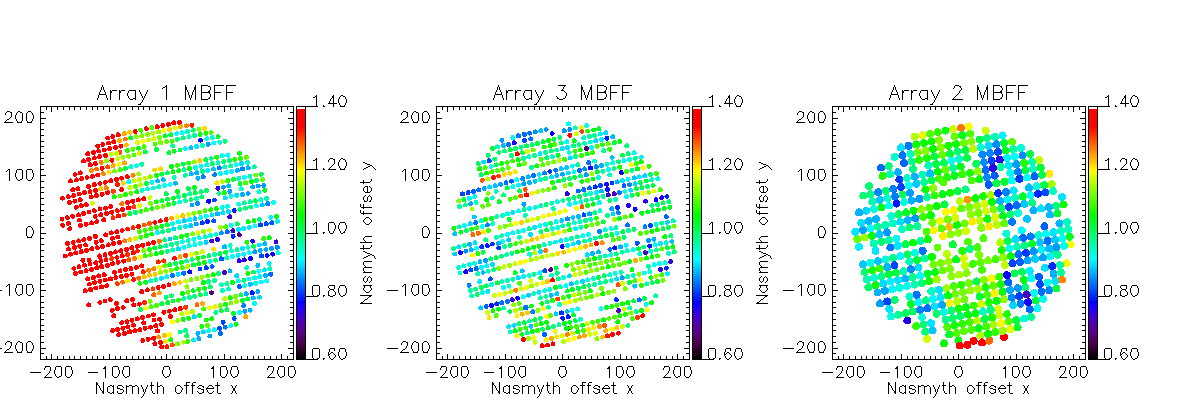
\includegraphics[width=0.95\textwidth]{Figures/Average_main_beam_flat_field_N2R9_10.png}
  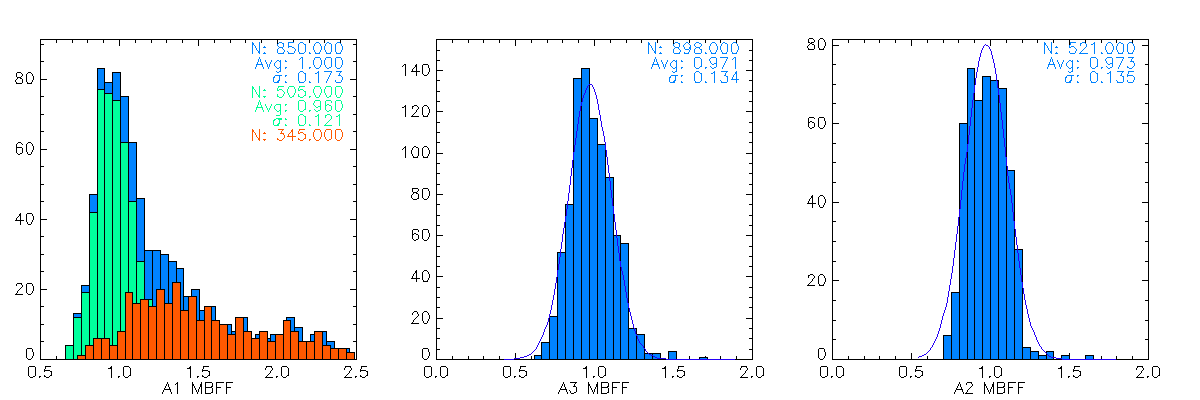
\includegraphics[width=0.8\textwidth]{Figures/Histo_average_main_beam_flat_field_N2R9_10.png}
\caption[Average main beam flat fields]{Average main beam flat fields
  obtained by combining the flat fields of five
  \bm\ scans. The top row plots show the normalized average flat fields of Array
  1, 3 and 2, respectively. {\lp The offset positions with respect to the center of
  the array are given in arcsecond in the Nasmyth coordinate
  system. The color code gives the value of the KID calibration
  coefficients, as defined in Eq.~\ref{eq:kid_gain}, normalized by the
  average calibration coefficient over all the
  KIDs of the array.} The bottom plots
  show the average flat field distributions using all KIDs (blue),
  using Array 1 KIDs that are positioned out of the shadow zone
  (green) and using Array 1 KIDs inside the shadow zone, which is
  defined in the text.}
 \label{fig:avg_mbff}
\end{center}
\end{figure*}

The dispersion of the detector responsivity across the field of view (\aka\ flat
fields) has been characterized in the following ways.

\noindent \emph{Main beam flat fields.} These are the focal plane
distribution of the calibration coefficients per KID. {\lp They describe the
focal plane distribution of the point spread function (PSF) in
the far field of the telescope.} The calibration coefficients $G_k$ are
estimated using Eq.~\ref{eq:kid_gain}, as discussed in
Sect.~\ref{se:practical_calib}. 

\noindent \emph{Forward beam flat fields.} These are the focal plane
distributions of the relative response of
each KID to the near field atmospheric background. They are estimated
using the correlation factor of each detector TOI 
to a median common mode estimated off-source (see Sect.~\ref{se:toi_proc} for
more details on common modes).

Figure~\ref{fig:avg_mbff} %and \ref{fig:avg_fbff}
shows the average main beam %and forward beam
flat field for the three arrays. These have been constructed by
combining the normalized flat fields of five \bms\ acquired during two
technical observation campaigns. These data were
selected by thresholding the line-of-sight opacity measured in the
1\,mm band to $\taunu\,x \leq 0.85$. The distributions for the average flat
fields are shown in the bottom panel of Fig.~\ref{fig:avg_mbff}.% and \ref{fig:avg_fbff}.

We observe a significant variation of the flat fields for A1 from the left-most side
to the right-most side of the FOV. This reveals a significant change of A1
detector responsivities depending on their position in the focal plane. Namely, this
effect mainly impacts the left-most third of the array, which is
referred to as the "shadow-zone''. This variation of the
flat field translates into a broadening of the distribution shown in
the lower panel of Fig.~\ref{fig:avg_mbff}.  However,
we verified that A1's flat field dispersions are in line with the ones of A3 after the
detectors within the shadow-zone were flagged out using a
crescent-shaped mask. The masked flat field distributions are shown in
green in Fig.~\ref{fig:avg_mbff}, %and \ref{fig:avg_fbff}
whereas shadow-zone distributions are in red. The same FOV patterning
is also observed in the forward beam flat fields, which excludes a
main beam related issue. 

%In addition to the average flat fields, we further
%characterize the flat fields for individual \bms. Fig.~\ref{fig:stddev_ff}
%shows the dispersion of the flat fields for nine \bms\ using
%either the whole FOV or masking the shadow-zone. The dispersion estimates for
%this two cases are gathered in Table~\ref{tab:flatfield_res}.
%While the
%shadow zone is exluded, the A1 flat field dispersions are reduced by a
%factor of about two, and reached values close to that of the A3 flat
%field dispersions, while the latters are unchanged. 

%\begin{table}[!h]
%\begin{center}
%\begin{tabular}{|l|l|c|c|c|}
%\hline
% Dispersion ($\%$)    & KID selection  &  A1 & A3  & A2 \\
%\hline
%Main beam flat field  & all the FOV           & $34.4 \pm 3.4$    & $15.5 \pm 1.4$  &  $13.2 \pm 1.7$  \\
%                      & shadow-zone excluded  & $17.0 \pm 1.1$    & $14.2 \pm 1.2$  &  $12.8 \pm 1.3$\\
%\hline
%Forward beam flat field  & all the FOV           & $21.6 \pm 1.4$  & $10.1 \pm 1.7$  & $5.2 \pm 0.9$   \\
%                         & shadow zone excluded  & $12.2 \pm 1.6$  & $10.1 \pm 2.1$  & $4.9 \pm 1.2$ \\
%\hline
%\end{tabular}
%\caption[Flat field dispersions]{Average flat field dispersions in percent for
%  nine \bms\ over all the FOV and after masking out the shadow-zone}
%\label{tab:flatfield_res}
%\end{center}
%\end{table}

%\begin{figure*}[!thbp] 
%\begin{center}
%  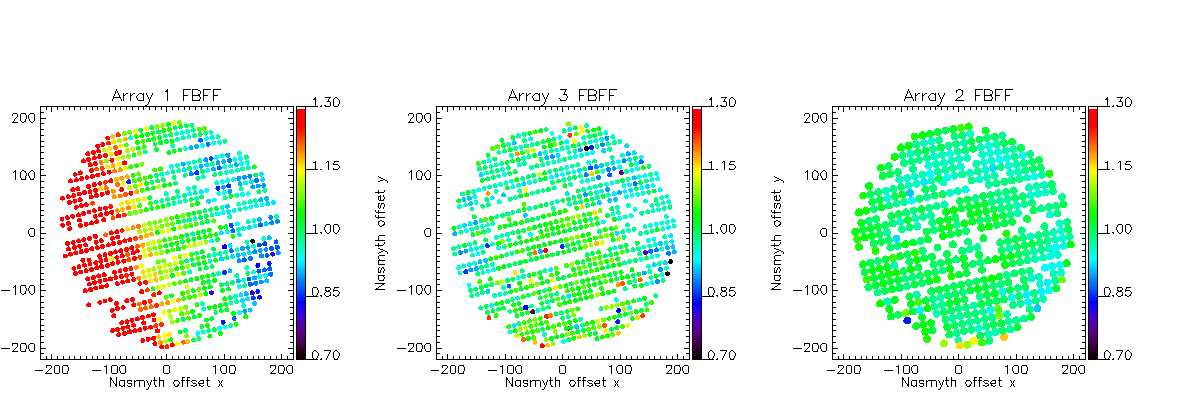
\includegraphics[width=0.95\textwidth]{Figures/Average_near_beam_flat_field_N2R9_10.png}
%  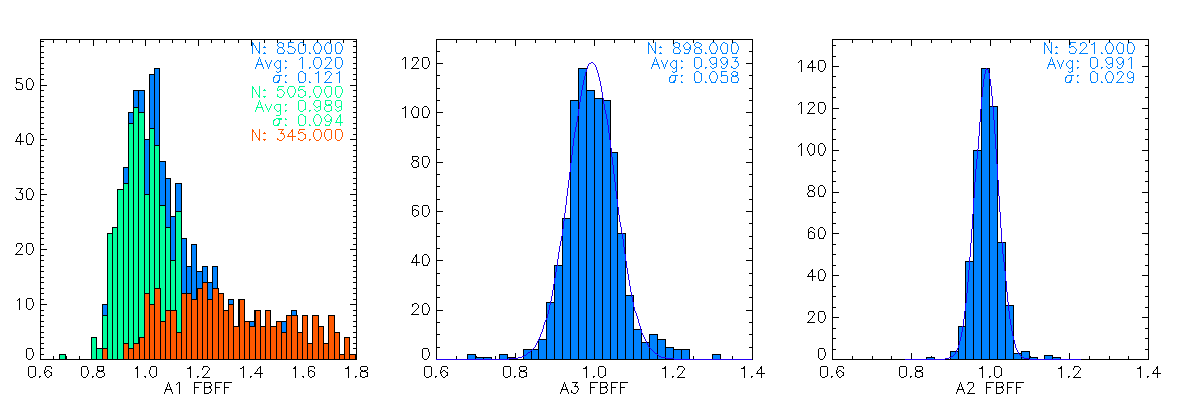
\includegraphics[width=0.8\textwidth]{Figures/Histo_average_near_beam_flat_field_N2R9_10.png}
%\caption[Average forward efficiency flat fields]{Average forward efficiency flat field for array 1, 3 and
%  2. Same legend as Fig.~\ref{fig:avg_mbff}}
% \label{fig:avg_fbff}
%\end{center}
%\end{figure*}

%\begin{figure}[ht] 
%\begin{center}
%  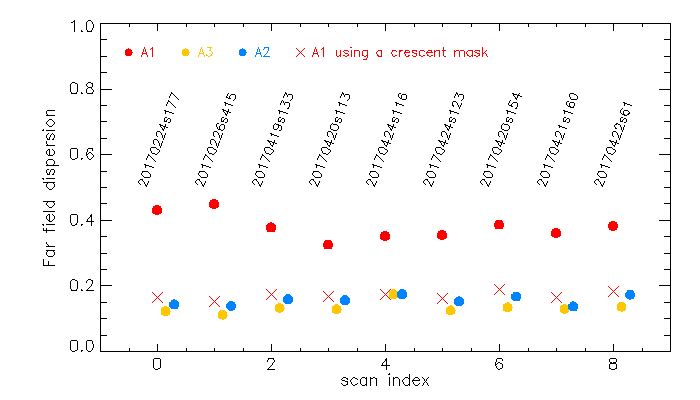
\includegraphics[width=0.6\textwidth]{Figures/FlatFields/Dispersion_main_beam_flat_field_N2R9_10_.png}
%  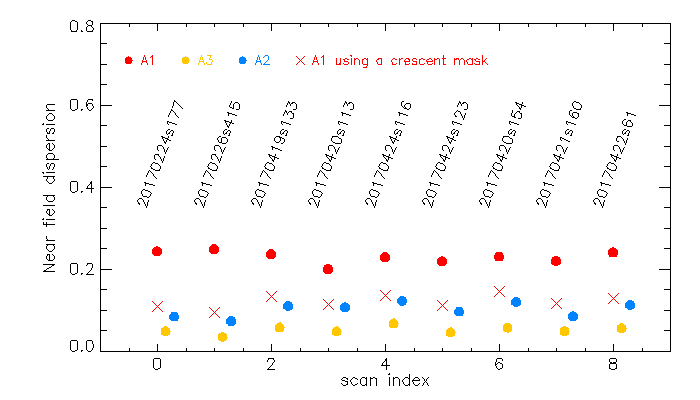
\includegraphics[width=0.6\textwidth]{Figures/FlatFields/Dispersion_forward_beam_flat_field_N2R9_10_.png}
%\caption[Dispersion of the flat field for nine \bms.]{The RMS
%  dispersion of the normalised main beam flat field (upper panel) and forward beam flat
%  field (lower panel) are shown using all valid KIDs of Array 1 (red circles),
%  Array 3 (orange circles) and Array 2 (blue circles), and using the KIDs
%  located outside the Array 1 "shadow zone'', which was discarded using a left
%  crescent-shaped mask (red crosses).}
% \label{fig:stddev_ff}
%\end{center}
%\end{figure}

The shadow zone effect is caused by {\lp a misbehaving of the dichroic in
the polarized transmission which is out of specifications. As a
result, the $1\,\rm{mm}$ polarisation that illuminates A1 is
attenuated.}
This effect,
which implies %a wrong placement of the transition zone of the dichroic
%that depends on frequency, incidence angle and polarisation,
{\lp a dependence of the frequency cut-off on the radiation
incidence angle and linear polarisation,}
was reproduced using optical simulations. Furthermore, this hypothesis was
verified using observations at the technical campaign of September
2018. During this test campaign, a new \emph{hot-pressed} dichroic had
been installed in place of the current \emph{air-gap} dichroic.
%
%Whereas the latter is made of a series of thin
%micron-like membranes separated by calibrated rings and mounted on
%a native ring in inox, the new hot-pressed dichroic consisted of a
%rigid disk of plastic with a thickness of about $2\,\rm{mm}$ mounted on a
%plastic ring.
%
The shadow zone variations of the flat field for A1 were
not observed during the September 2018 campaign, while huge distortions
across the field of view of A2 were reported. These distortions are
due to the bending of the hot-pressed dichroic at low temperature.
This test has confirmed that the shadow zone effect was due
to incoming radiation absorption by the current air-gap dichroic.
Further efforts are currently conducted to the design of a dichroic that
combines robustness against bending induced by low temperature and
optimal transmission.
{\lp The air-gap dichroic, which is immune to low temperature-induced
deformation, has been re-installed at the end of the September 2018
run coming back to the instrumental set up discussed in this paper. We
have checked that, as expected, the performance of the instrument
after this intervention was consistent with the one reported in this
paper.}


%---------------------------------------------------------------------
%	TEMPERATURE-INDUCED VARIATION
%---------------------------------------------------------------------
%\subsection{Temperature-induced variations of the beam}
\subsection{The temperature-induced variation effect}
\label{se:beam_variation}

We evidenced a daily variation of the flux density estimates that correlates to the
measured beam size. This beam broadening happens mostly in afternoons and around
sunrise and sunset. It is also reproducible from one campaign to another. It most certainly
comes from the combination of two different effects.

First inhomogeneous solar illumination leads to large scale deformations of the
\trentemetre\ primary mirror, which in turn lead to variable de-focussing of the
telescope. {\lp To mitigate this effect, the telescope is equipped with an
  active thermal ventilation system of the primary mirror and an active
  temperature control of the secondary support legs. This system is, however,
  challenged when the Sun partially illuminates the telescope}
  %, like around
  %sunrise and sunset.}
  {\lp This is a known effect that also impacts
  observations with the heterodyne instruments operated at the IRAM
  \trentemetre\ telescope. It had also been already observed with the previous
  generation total-power instruments MAMBO-2 \citep{Kreysa1999}.} However, the
magnitude of this effect is likely to have increased with the slow disappearance
of the surface painting of the primary mirror in the past few years.

Second, on short time scales, atmospheric anomalous refraction {\lp also often plays a
  role.}. As far as the \trentemetre\ telescope is concerned, it has first
been described in~\citet{Altenhoff1987}. Based on experience with
  the heterodyne receivers, afternoon hours are
  often affected with an unstable atmosphere when rising moist air moves
  through the beam of the telescope and causes random refraction. The pointing
  is then observed to change within few seconds by few arcseconds {\lp resulting in an average
    enlargement of the beam pattern.} This effect has been confirmed by
  measuring several arcsec displacements of the source position when projected using
  different subsets of subscans of a single observation, as described
  in Appendix~\ref{ap:beam_monitoring}. We find that the apparent beam broadening during
  the afternoon is due to anomalous refraction for between one third
  and one half of the scans over the period studied here.


{\lp As both effects (the primary mirror deformations and the anomalous
  refraction) are due to ambiant temperature variations, we refer to them as
  \emph{temperature-induced variation effects} in the following.}\\
%% The impact of these effects on the flux density estimates can be
%%   mitigated, as explained below in
%%   Sects.~\ref{se:baseline_calibration}-\ref{se:photometric_correction}, provided
%%   the beam size variations are accurately monitored. Here, we describe the
%%   methods that are used for this monitoring.


\begin{figure}[ht!]
  \begin{center}
    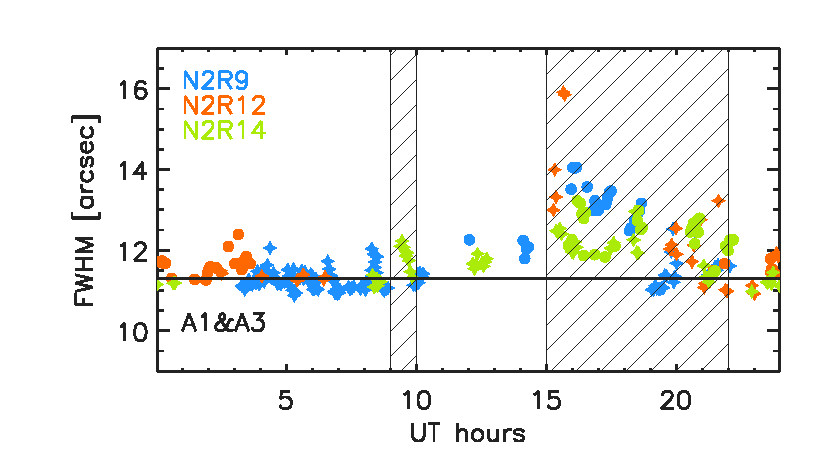
\includegraphics[clip=true, trim={0.9cm, 0.5cm, 0.5cm, 0.5cm}, width=0.4725\textwidth]{Figures/Beam_monitoring_with_otfs_vs_ut_1mm.pdf}
    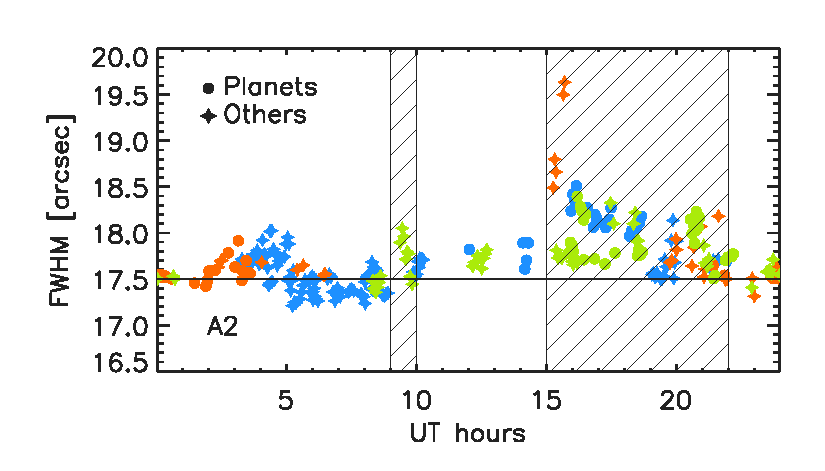
\includegraphics[clip=true, trim={0.5cm, 0.5cm, 0.5cm, 0.5cm}, width=0.4875\textwidth]{Figures/Beam_monitoring_with_otfs_vs_ut_a2.pdf}
    \caption[Beam size monitoring using OTF scans]{Beam size
      monitoring using OTF raster scans. Geometrical FWHM at $1\,\rm{mm}$ (top panel)
      and $2\,\rm{mm}$ (bottom panel), as a function of the
      observation time in UT hours, are shown using scans of giant
      planets (filled circles) and bright point-like sources with a
      flux density higher than $1\,\rm{Jy}$ (filled stars) for the three \emph{reference}
      observation campagns (N2R9,N2R12 and N2R14). The cross-hatched areas
      correspond to the observing time periods that are discarded using
      the \emph{baseline} scan selection, as described in Sect.~\ref{se:data_selection}.} 
\label{fig:beam_monitoring_otf}
  \end{center}
\end{figure}

%% \subsubsection{Beam monitoring using bright source scans}
%% \label{se:beam_monitoring_otf}

The temperature-induced variation of the beam size as a function of
the UT hours is shown in Fig.~\ref{fig:beam_monitoring_otf} for the
three reference campaigns using bright sources. These are
selected by thresholding the flux density estimates above $1\,\rm{Jy}$
at both wavelengths. The beam size is estimated by fitting a 2D
elliptical Gaussian to the map {\lp and computing the geometrical FWHM
using Eq.~\ref{eq:fwhm_geom}.} For the resolved planet as Uranus, the
FWHM estimates are corrected for the beam broadening due to the finite
extension of the apparent disc of the planet, as in
Sect.~\ref{se:mainbeam}.
We observe the same evolution of
the FWHM for all campaigns. 
This goes from a plateau at a median value of $11.3''$ at $1\,\rm{mm}$
and $17.5''$ at $2\,\rm{mm}$ during the night, to a smooth rise that
reaches a maximum of about $14''$ at $1\,\rm{mm}$ and $18.5''$ at
$2\,\rm{mm}$ around 16:00 UT hours. The beam broadening becomes large
around 15:00 UT and returns to the plateau only around 22:00 UT.
To mitigate the impact of the temperature-induced variation,
observation scans acquired during this time interval must be
discarded. The UT ranges that are discarded
using the \emph{baseline} scan selection (see
Sect.~\ref{se:data_selection}) are shown as cross-hatched areas in
Fig.~\ref{fig:beam_monitoring_otf}.
They consist of the afternoon
period between 15:00 and 22:00 UT %, which corresponds to the period
%when the daylight heating of the telescope primary mirror has the most
%impact,
as well as the period from 9:00 UT to 10:00 UT while the Sun
rises. 
%This leads to discard scans belonging to the cross-hatched intervales
%for the \emph{baseline} scan selection (Sect.~\ref{se:data_selection}
%and \ref{se:baseline_calibration}).
{\lp Whereas the global trend of the beam variations is the
same for all campaigns, we observe some variability in the amplitude
of the effect over the campaigns. This supports the assumption of the
important role of the partial illumination of the primary mirror by
direct sun light in the temperature-induced effect. This in turn
induces a variability of the amplitude of the effect depending on the
angle between the telescope boresight % telescope optical axis
and the Sun all along the
observations.}

The same beam size variations in time are observed using scans of giant planets
(Uranus and Neptune) or other bright
sources (mainly quasars). However, planets lead slightly larger FWHM
estimates than quasars, because of
%the non negligible coupling of the flux to the error beams.
the larger contribution of the error beams to the fitted 2D Gaussian,
as their flux are measured with a higher signal-to-noise.
%in the case of bright sources.
%the non negligible coupling of their flux to the error beams.

%{\lp The global trend of the beam variations is the same for all campaigns, but
%  indeed, variations are observed, certainly following the differences in
%  outside temperature and precise primary illumination between different scans.}
%Last, among the presented scans, planets lead slightly larger beams than
%quasars, because of the non negligible coupling of their flux to the error beams.

%% The same beam size variations in time using scans of giant planets
%% (Uranus and Neptune) or other bright
%% sources (mainly quasars) are observed. However, the FWHM from planet %FWHM$_{\rm{geom}}$ from planet
%% observations tend to be slightly larger than those from observations
%% of other sources. {\lp For example, most of the planet FWHM estimates
%% are above the median FWHM calculated using the scans acquired during the
%% night, which are shown as horizontal lines in Fig.~\ref{fig:beam_monitoring_otf}.}
%% {\lp This originates from the larger contribution of the
%% error beams to the fitted 2D Gaussian, as flux are measured with 
%% %larger 2D Gaussian fitted
%% %values due to the error beams, which are measured with
%% a higher signal-to-noise in the case of bright sources.} This small
%% effect is accounted for in the beam-dependent calibration cross-check
%% discussed in Sect.~\ref{se:photometric_correction}.

%% \subsubsection{Beam monitoring using pointing}
%% \label{se:beam_monitoring_pointing}
%% 
%% For a finer sampling of the observation time, we also consider using
%% the pointing scans for beam monitoring. As discussed in
%% Sect.~\ref{se:pointing}, the telescope pointing is
%% monitored on a hour basis during observation using {\tt pointing}
%% scans. As these scans consist of two sub-scans in azimuth and
%% elevation of about 10 seconds of integration time each, they
%% can also be used to make a map of the pointing source. For each campaign,
%% we thus have on hands hundreds of maps of mostly point-like bright
%% sources, which can also be used to monitor the beam size. However, we
%% expect less accuracy than using standard OTF raster
%% scans of bright sources due to the shorter integration time and the
%% fact that only the centermost KIDs in the array see the source.  
%% 
%% %traitement pointing scans
%% For this purpose, {\tt pointing} scans are reduced using
%% the data analysis pipeline described in
%% Sect.~\ref{se:dataproc} with the same parameters as for
%% standard OTF raster scans, and projected onto maps of $2''$ resolution.
%% As previously, an elliptical 2D Gaussian is then fitted from the map
%% and the geometrical FWHM%$_{\rm{geom}}$
%% %is formed from the best-fit FWHM along the two axis.
%% is computed.
%% %FWHM estimates on Uranus maps are corrected for an
%% %offset due to the finite size of the apparent disc, as discussed in
%% %Sect.~\ref{se:beam_monitoring_otf}.
%% {\tt Pointing} scans on {\lp slightly extended} sources, such as NGC7027,
%% are discarded from the analysis.
%% 
%% 
%% % anomalous refraction
%% For each {\tt pointing}, we also seek for signs of atmospheric anomalous refraction. There are
%% enough KIDs per observation band to make an independent map using only
%% one subscan, i.e. 10 seconds of integration time.
%% For each of the four cross subscans, we thus estimate the position of the best
%% 2D Gaussian that fits the map. We compute the deviation between each
%% subscan-derived position and the best-fit position using the entire
%% scan. An anomalous refraction event is detected when the difference is
%% above $2.5''$ for at least one subscan. We find that the apparent beam
%% broadening during the afternoon is due to anomalous refraction for
%% between one third and one half of the scans over the period studied
%% here.
%% %\footnote{See the study posted
%% %  in the commissioning internal wiki at
%% %  \url{http://www.iram.fr/wiki/nika2/index.php/Millimetric_anomalies_(weather,_antenna)_as_monitored_by_pointing_scans}}.
%% %} 
%% 
%% %In Fig.~\ref{fig:beam_monitoring_pointing}, we present the FWHM
%% %estimates using pointing scans as a function of the observing time in
%% %UT hours for three observation campaigns. We observe the same beam
%% %size evolution with UT hours as previously discussed in
%% %Sect.~\ref{se:beam_monitoring_otf}, that is a plateau during night-time
%% %and a smooth increase during day-time up to a maximum in the
%% %afternoon, which is followed by a smooth decrease down to the plateau
%% %a few hours after the sunset. Although the general trend is the same
%% %as the OTF-based FWHM variations, more dispersion is seen either using
%% %pointings toward giant planets or other bright sources.
%% %
%% %\begin{figure}[ht!]
%% %  \begin{center}
%% %    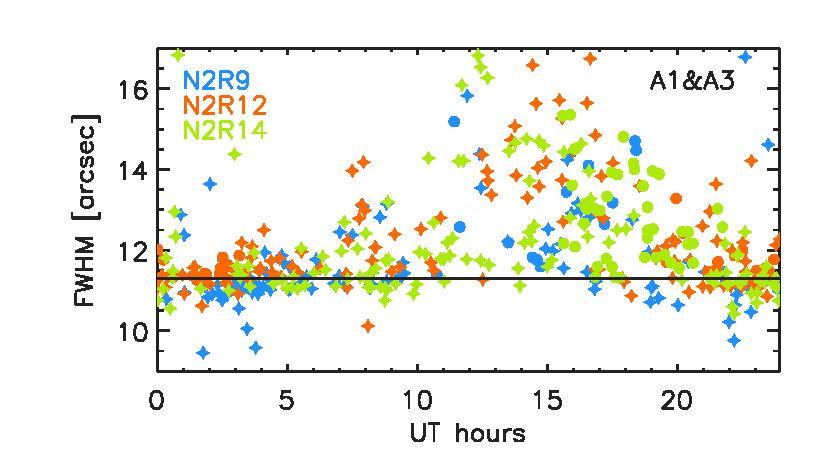
\includegraphics[clip=true, trim={0.9cm, 0.5cm, 0.5cm, 0.5cm}, width=0.4725\textwidth]{Figures/Beams/Beam_monitoring_with_pointings_vs_ut_1mm.pdf}
%% %    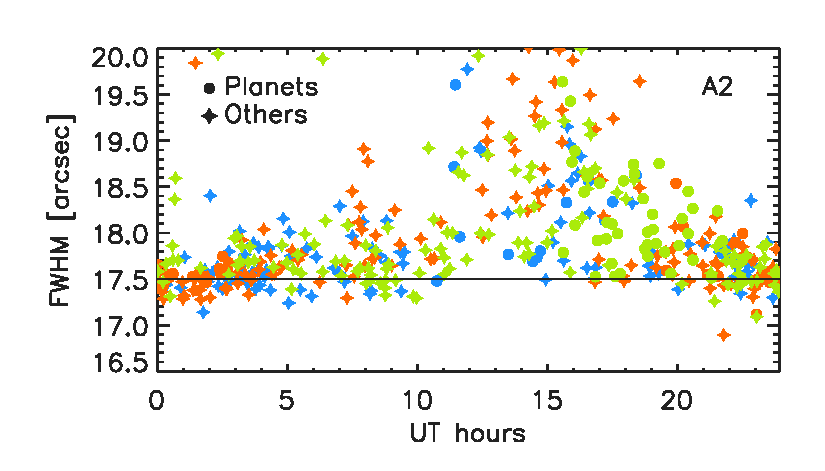
\includegraphics[clip=true, trim={0.5cm, 0.5cm, 0.5cm, 0.5cm}, width=0.4875\textwidth]{Figures/Beams/Beam_monitoring_with_pointings_vs_ut_a2.pdf}
%% %    \caption[Beam size monitoring using pointing scans]{Beam size
%% %      monitoring using pointing scans. Same legend as in
%% %      Fig.~\ref{fig:beam_monitoring_otf}.} 
%% %\label{fig:beam_monitoring_pointing}
%% %\end{center}
%% %\end{figure}
%% %
%% The pointing-based FWHM estimates constitute a time-sampling of the
%% beam size during
%% the whole observation campaign. They can serve to estimate the beam
%% size of any observation scans, in particular
%% toward sources too faint for a direct FWHM %$_{\rm{geom}}$
%% fit to be made on the map. To mitigate the dispersion, the time-stamped
%% pointing-based FWHM
%% %$_{\rm{geom}}$
%% is filtered with a running median on a 70-minute
%% width time window. Then, the FWHM %$_{\rm{geom}}$
%% at the time of the considered scans is
%% interpolated from the median-filtered pointing-based FWHM.%$_{\rm{geom}}$.
%% %
%% \begin{figure}[ht!]
%%   \begin{center}
%%     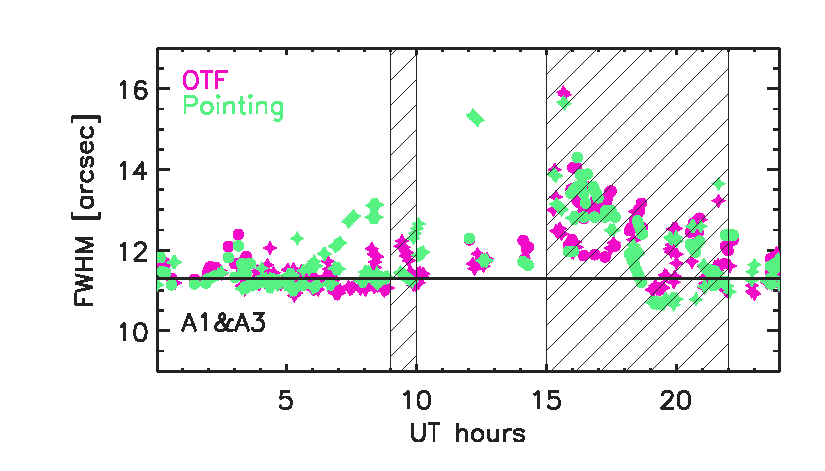
\includegraphics[clip=true, trim={0.9cm, 0.5cm, 0.5cm, 0.5cm}, width=0.4725\textwidth]{Figures/Beam_monitoring_with_otfs_vs_ut_compare_pointings_1mm.pdf}
%%     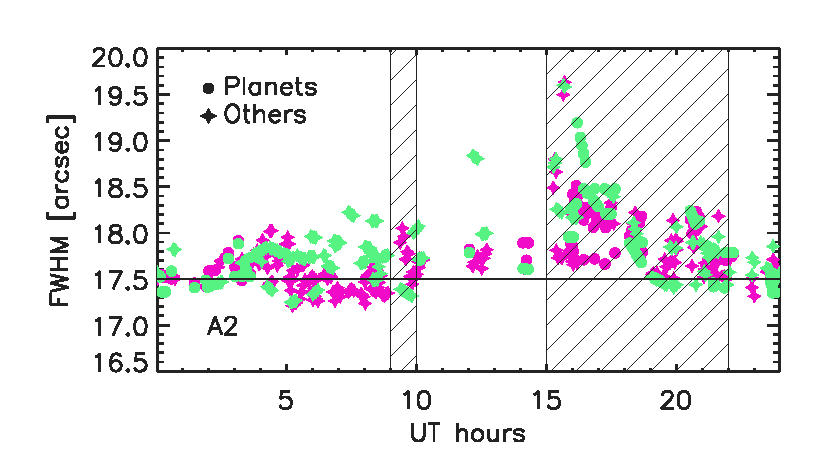
\includegraphics[clip=true, trim={0.5cm, 0.5cm, 0.5cm, 0.5cm}, width=0.4875\textwidth]{Figures/Beam_monitoring_with_otfs_vs_ut_compare_pointings_a2.pdf}
%%     \caption[Beam size monitoring comparison]{Beam size monitoring.
%%      'OTF'-labeled pink data points show the FWHM estimates from a 2D
%%     Gaussian fit on the maps of OTF raster scans towards bright
%%     sources, whereas the 'Pointing'-labeled light green data points
%%     are FWHM estimates obtained by interpolating the {\lp
%%     median-filtered} pointing-based FWHM at the time of the
%%     scans. {\lp The
%%     pointing-based FWHM estimates are obtained by fitting a 2D Gaussian on the
%%     maps of {\tt pointing} scans.}}
%% \label{fig:beam_monitoring_compare}
%% \end{center}
%% \end{figure}
%% %
%% Figure~\ref{fig:beam_monitoring_compare} shows two different FWHM %$_{\rm{geom}}$
%% estimates for the same data set: on one hand the best-fit FWHM %$_{\rm{geom}}$
%% estimates on the OTF-scan map and on the other hand the interpolation from
%% the pointing-based FWHM %$_{\rm{geom}}$
%% monitoring. The two estimates show the same global variations as a
%% function of the UT hours. They are well in agreement with each
%% other, although the pointing-based estimates have more dispersion and
%% a few outliers.
 
%As a summary, we have evidenced a systematic beam size variation with
%the observation time using two different data sets: a series of OTF
%scans of bright sources and pointing scans. The beam size
%variation is i) reproducible from a campaign to another, stable
%with ii) the data set and iii) the sources. It consists of a beam
%broadening during afternoons and an increase of the dispersion during
%sunrises. \new{The \afternoon\ beam-size variation effect mainly
%originates from deformations of the $30\,\rm{m}$ primary mirror subject
%to the Sun irradiation, while anomalous refraction also play a
%role.}  
%The most impacted
%observing periods are well discarded using the baseline selection
%criteria discussed in Sect.~\ref{se:data_selection}.


%*************************************************************************
%
%   SEE CALIBRATION_2 FOR THE SECOND PART
%
%************************************************************************


%---------------------------------------------------------------------
%	BASELINE CALIBRATION
%---------------------------------------------------------------------
%\subsection{Baseline calibration}
%\label{se:baseline_calibration}



%---------------------------------------------------------------------
%	PHOTOMETRIC CORRECTION
%---------------------------------------------------------------------
%\subsection{Photometric correction}
%\label{se:photometric_correction}
